\begin{frame}[c]{}

\centering
\huge
Lecture 2:\\
Design Spaces in Machine Learning
\end{frame}
%----------------------------------------------------------------------
%----------------------------------------------------------------------
\begin{frame}[c]{Where are we? The big picture}

\begin{itemize}
	\item Introduction
	\item[$\to$] Background
	\begin{itemize}
		\item[$\to$] Design spaces in ML
		\item Evaluation and visualization
	\end{itemize}
	\item Hyperparameter optimization (HPO)
	\begin{itemize}
	  \item Bayesian optimization
	  \item Other black-box techniques
      \item Speeding up HPO with multi-fidelity optimization
	\end{itemize}
	\item Pentecost (Holiday) -- no lecture
	\item Architecture search I + II
	\item Meta-Learning
	\item Learning to learn $\&$ optimize
	\item Beyond AutoML: algorithm configuration and control
	\item Project announcement and closing
\end{itemize}


\end{frame}
%----------------------------------------------------------------------
%----------------------------------------------------------------------
\begin{frame}[c]{Learning Goals}

After this lecture, you will be able to \ldots

\begin{itemize}
  \item identify design decisions of machine learning algorithms
  \item explain different types of design decisions and there relations
  \item create design spaces
  \item discuss the pros and cons of different design space approaches
  \item explain design spaces for neural architecture search
\end{itemize}

\end{frame}
%----------------------------------------------------------------------
%----------------------------------------------------------------------
\begin{frame}[c]{Simple Design Decisions: Selection of Algorithm}

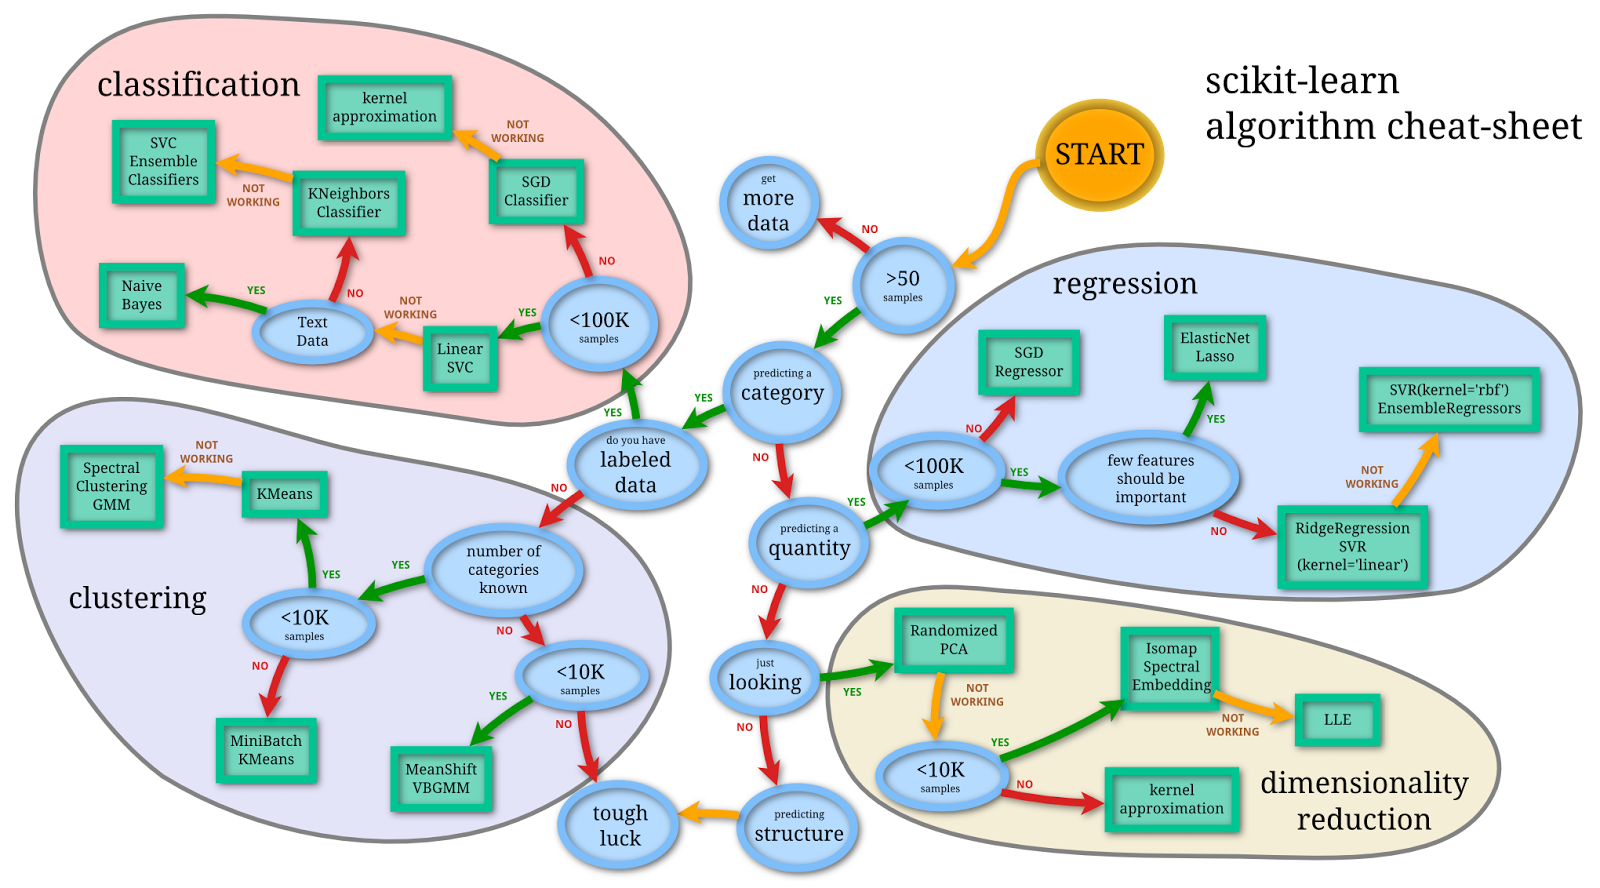
\includegraphics[width=1.0\textwidth]{images/sklearn-cheat}


\end{frame}
%----------------------------------------------------------------------
%----------------------------------------------------------------------
\begin{frame}[c]{Simple Design Decisions: Selection of Algorithm}

\begin{itemize}
  \item categorical design decison: $\{ \algo_1, \algo_2, \algo_3, \ldots, \algo_n\}$
  \begin{itemize}
	\item random forest (RF), support vector machine (SVM),\\ gradient boosting (GB), \ldots
    \item there is no ordering between algorithms
    \item set notation
  \end{itemize}
  \pause
  \item if we would run all of them and each takes (on average) $t$ seconds:\\
  $t \cdot n$ seconds
  \pause
  \smallskip
  \item in addition, choose pre-processing algorithm: $\{\algo_1^P, \algo_2^P, \algo_3^P, \ldots \algo_l^P \}$
  \begin{itemize}
    \item PCA, feature selection, random kitchen sinks, \ldots
  \end{itemize}
  \item if we only use one preprocessor and one ML algorithm,\\ exhaustive search would require:
  $t \cdot n \cdot l$
\end{itemize}

\end{frame}
%----------------------------------------------------------------------
\section{Design Space from Documentation}
%----------------------------------------------------------------------
\begin{frame}[c]{Design Space of Support Vector Machines}

\centering
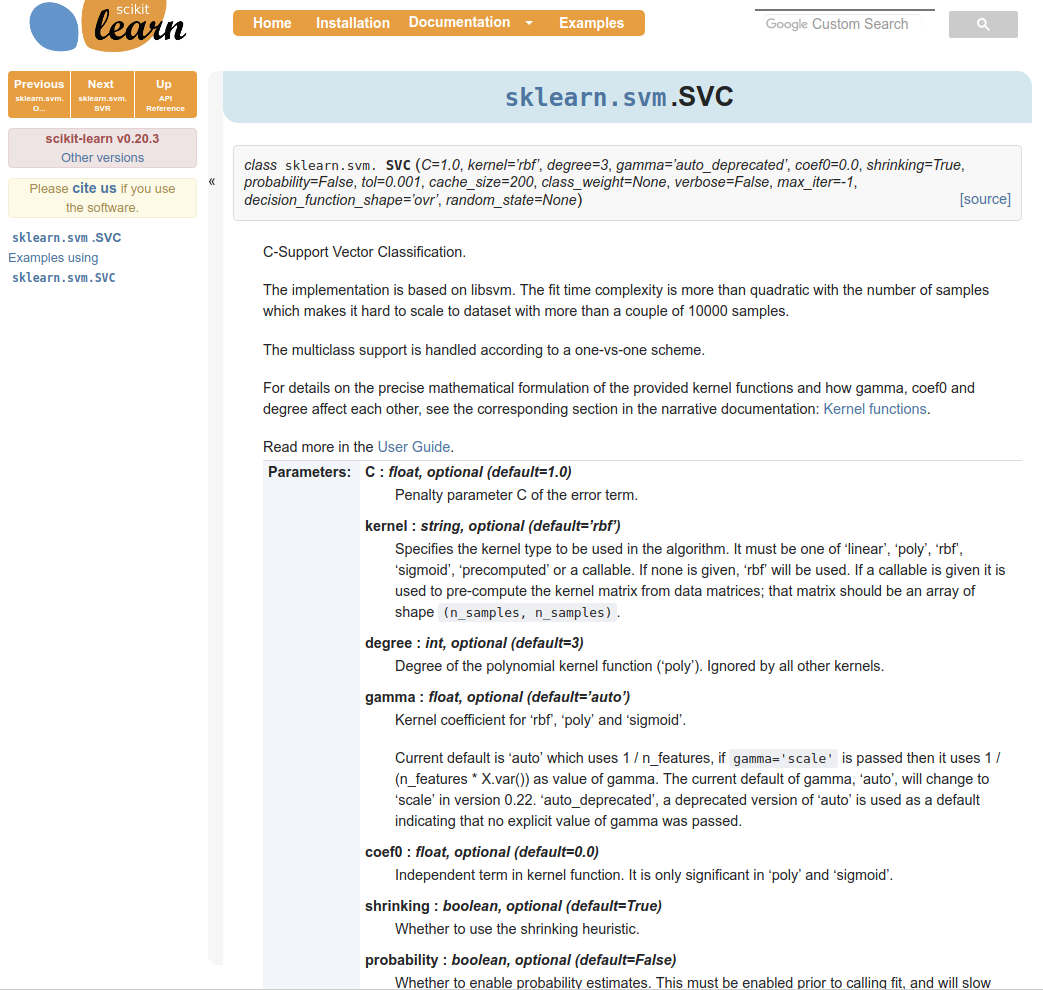
\includegraphics[width=0.7\textwidth]{images/sklearn_svm_doc.png}

\end{frame}
%----------------------------------------------------------------------
%----------------------------------------------------------------------
\begin{frame}[c]{Design Space of Support Vector Machines}

\begin{block}{Hyperparameter Optimization (HPO; informal)}
Given
\begin{itemize}
  \item a dataset
  \item a set of hyperparameters of a machine learning algorithms
  \item a cost metric (e.g., predictive error)
\end{itemize}
we want to find the hyperparameter configuration\\ that minimizes the cost metric wrt the dataset. 
\end{block}

\begin{block}{Hyperparameter Types of SVM}
\begin{description}
  \item[C] float hyperparameter
  \item[Kernel] categorical hyperparameter
  \item[Degree] integer hyperparamerter
  \item[gamma] float hyperparamerter
  \item \ldots
\end{description}
\end{block}

\end{frame}
%----------------------------------------------------------------------
%----------------------------------------------------------------------
\begin{frame}[c]{Hyperparameter Types}

\begin{description}
	\item[categorical] set of values (not sorted) with uniform distance
	\begin{itemize}
	  \item \texttt{kernel \{linear, rbf, poly, sigmoid\}}
	\end{itemize}
	\pause
	\item[ordinal] list of ordered values with uniform distance between neighbors
	\begin{itemize}
	  \item no example in SVM design space
	  \item \texttt{size [small, medium, large]}
	\end{itemize}
	\pause
	\item[integer] bounded range of integers
	\begin{itemize}
	  \item \texttt{degree [1, 5]}
	\end{itemize}
	\pause
	\item[float] bounded range of floats
	\begin{itemize}
	  \item \texttt{gamma\_value [0.0001, 8.0]}
	\end{itemize}
\end{description}

\end{frame}
%----------------------------------------------------------------------
%----------------------------------------------------------------------
\begin{frame}[c,fragile]{Design Space and Configuration}

\begin{block}{Design/Configuration Space}
The combination of several hyperparameter ranges $\pcs_i$ for the $i$-th hyperparameter creates a design space:
$\pcs = \pcs_1 \times \pcs_2 \times \pcs_3 \ldots \times \pcs_n$ 

\pause
\bigskip

For example, the design space of a SVM would include:

\begin{verbatim}
kernel categorical {linear, rbf, poly, sigmoid}
degree integer [1, 5]
gamma_value float [0.0001, 8.0]
\end{verbatim}
\end{block}

\pause

\begin{block}{Configuration}
An element of the configuration space $\conf \in \pcs$ instantiates each hyperparameter $\conf_i$ with a value.
For example:
\begin{verbatim}
{kernel: rbf, gamma_value: 1, degree: 2}
\end{verbatim}

\end{block}

\end{frame}
%----------------------------------------------------------------------
%----------------------------------------------------------------------
\begin{frame}[c]{Concept of Defaults}

\begin{itemize}
  \item We assume that each algorithm has a default
  \begin{itemize}
    \item often a robust configuration if you don't want to change it
    \item defaults often provided by developer, e.g.,\\
   		  in its documentation or the corresponding paper
  \end{itemize}
  \pause
  \item We use the default to start our search for HPO
  \begin{itemize}
    \item if we know a reasonable configuration,\\ we should start with a random configuration?
    \item Goal: find something which is better than the default
    \pause
    \smallskip
    \item Pro: Can help us to start in good region of the design space
    \item Contra: We might start being trapped in local optimum.
  \end{itemize}
\end{itemize}

\pause
Example: the default \texttt{kernel} of the SVM could be the RBF-kernel\\
\texttt{kernel categorical \{linear, rbf, poly, sigmoid\}[rbf]}

\end{frame}
%----------------------------------------------------------------------
%----------------------------------------------------------------------
\begin{frame}[c, fragile]{Conditional Dependencies}

\begin{block}{SVM Example}
\begin{verbatim}
kernel categorical {linear, rbf, poly, sigmoid}[rbf]
degree integer [1, 5][3]
gamma_value float [0.0001, 8.0][2.0]
\end{verbatim}
\end{block}

\begin{itemize}
  \item Some hyperparameters depend on each other
  \begin{itemize}
    \item \texttt{degree} is only active if \texttt{kernel} is set to \texttt{poly}
    \item \texttt{gamma\_value} is only active if \texttt{kernel} is set to \texttt{rbf}  
  \end{itemize}
  \bigskip
  \pause
  \item[$\leadsto$] model such conditional dependencies in configuration space:
\end{itemize}

\begin{verbatim}
degree | kernel in {poly}
gamma_value | kernel in {rbf}
\end{verbatim}

\end{frame}
%----------------------------------------------------------------------
%----------------------------------------------------------------------
\begin{frame}[c, fragile]{Remarks (I): Conditional Dependencies}

\begin{block}{Duplicates of Hyperparameters?}
\begin{itemize}
	\item Sometimes algorithms have the same sub-hyperparameter\\ (with slightly different meanings)
	\item Two approaches:
	\begin{itemize}
		\item Duplicate hyperparameter and use conditionals \\
		$\leadsto$ larger configuration space
		\item a single hyperparameter\\
		$\leadsto$ optimizer has to learn dependencies on its own
	\end{itemize}
    \item Not well studied which way is better under which conditions
\end{itemize}
\end{block}
	
\end{frame}
%----------------------------------------------------------------------
%----------------------------------------------------------------------
\begin{frame}[c, fragile]{Remarks (II): Conditional Dependencies}

\begin{block}{Imputation}
	\begin{itemize}
		\item Inactive hyperparameters can be handled in different ways
		\item Most trivial approach: imputation of deactivated hyperparameters
		\begin{enumerate}
			\item Impute with default value
			\item Impute with non-existing value
		\end{enumerate}
		\pause
		\medskip
		\item Risk:
		\begin{itemize}
			\item confusing for some optimizers (in particular model-based optimizers)
		\end{itemize}
		\pause
		\item One of the open challenges: best way to handle conditionals
	\end{itemize}
\end{block}

\end{frame}
%----------------------------------------------------------------------
%----------------------------------------------------------------------
\begin{frame}[c, fragile]{Forbidden Constraints}

\begin{itemize}
  \item Combinations of settings can be forbidden
  \item For example: $a \leq b$
  \smallskip
  \pause
  \item[$\leadsto$] Try to avoid such constraints\\ because sampling in constrained spaces gets much harder
  \smallskip
  \item Sometimes constraints can be rewritten:
\end{itemize}

\begin{verbatim}
    a float [0,1][0]
    b float [0,1][0]
    a <= b
\end{verbatim}

Rewrite:
\begin{verbatim}
    a float [0,1][0]
    c float [0,1][0]
\end{verbatim}

with $b = a + c$ $\leadsto$ \texttt{b} might be larger than 1! 


\end{frame}
%----------------------------------------------------------------------
%----------------------------------------------------------------------
\begin{frame}[c, fragile]{Expert Knowledge: Transformations}

\begin{itemize}
	\item Expert knowledge can help to guide hyperparameter optimization
	\item For example, some hyperparameters might not be sampled uniformly
\end{itemize}

\pause
\medskip
For example, regularization hyperparameter of SVM:

\begin{verbatim}
    C float [0.001, 1000.0][1.0]
\end{verbatim}

\begin{itemize}
	\item the distance between $999.9$ and $1000.0$ should not be the same as between $0.001$ and $0.101$
	\smallskip
	\pause
	\item[$\leadsto$] We might want to sample here from from a log-scale
\end{itemize}

\begin{verbatim}
    C float [0.001, 1000.0][1.0] log
\end{verbatim}

\end{frame}
%----------------------------------------------------------------------
%----------------------------------------------------------------------
\begin{frame}[c]{Design Space of Support Vector Machines}

\centering
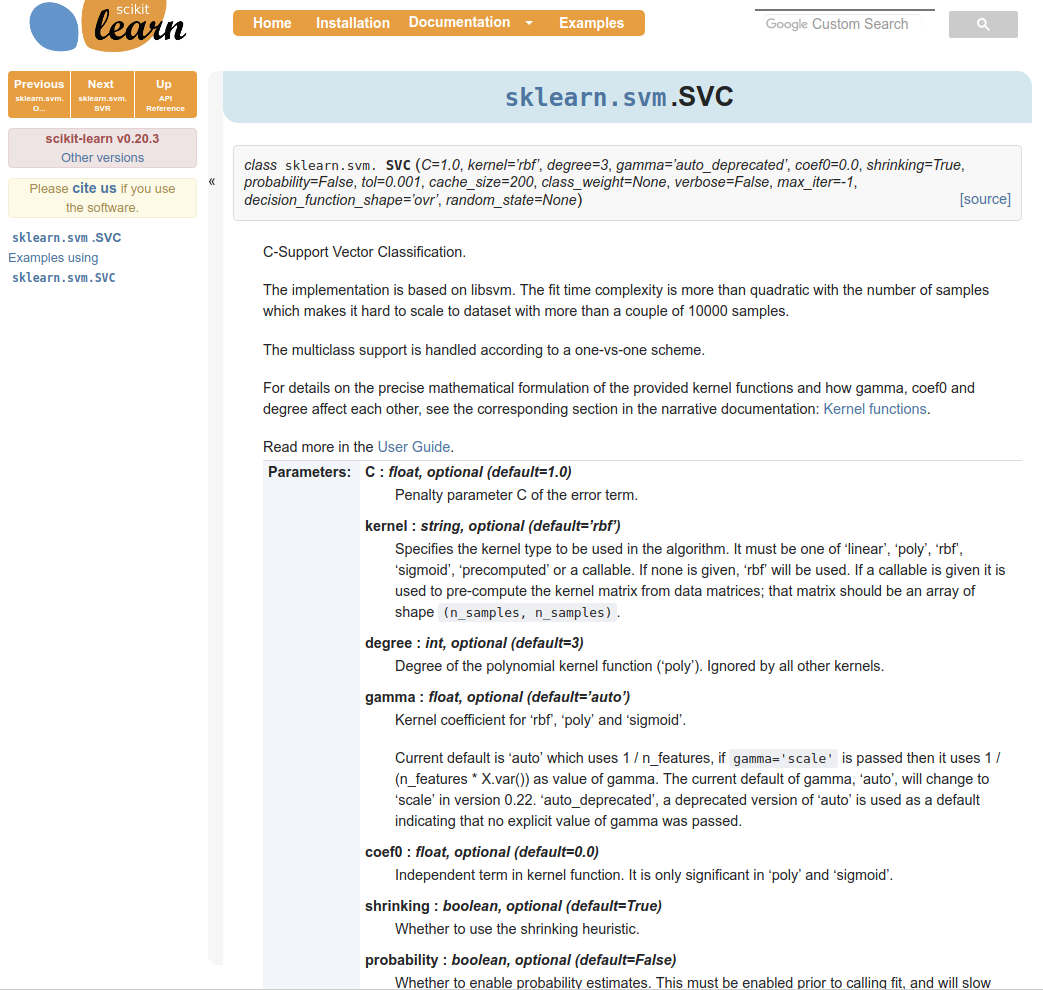
\includegraphics[width=0.7\textwidth]{images/sklearn_svm_doc.png}

\end{frame}
%----------------------------------------------------------------------
%----------------------------------------------------------------------
\begin{frame}[c, fragile]{Configuration Space of SVM}

\begin{verbatim}
  Hyperparameters:
    C float [0.001, 1000.0][1.0] log
    coef0 float [0.0, 10.0][0.0]
    degree integer [1, 5][3]
    gamma categorical {auto, value}[auto]
    gamma_value float [0.0001, 8.0][1.0]
    kernel categorical {linear, rbf, poly, sigmoid}[poly]
    shrinking categorical {true, false}[true]
  Conditions:
    coef0 | kernel in {poly, sigmoid}
    degree | kernel in {poly}
    gamma | kernel in {rbf, poly, sigmoid}
    gamma_value | gamma in {value}
\end{verbatim}

\end{frame}
%----------------------------------------------------------------------
%----------------------------------------------------------------------
\begin{frame}[c, fragile]{Optimization of Random Seeds?}

Is the random seed a valid design decision?

\medskip

\begin{block}{Output: trained model}
	If the output of your AutoML tool is a trained model:
	\begin{itemize}
		\item your goal is to obtain the best trained model
		\item[$\leadsto$] tune your random seed!
	\end{itemize}
\end{block}

\pause	
\medskip
	
\begin{block}{Output: best configuration}
	If the output of your AutoML tool is the best configuration:
	\begin{itemize}
		\item your goal is to obtain a configuration that performs well after refitting 
		\item[$\leadsto$] don't tune your random seed!
		\item[$\leadsto$] obtain configuration that performs well on many random seeds
	\end{itemize}
\end{block}


\end{frame}
%----------------------------------------------------------------------
\section{Design Space from Algorithm}
%----------------------------------------------------------------------
\begin{frame}[c]{Algorithm: Randomized Regression Tree}

\begin{algorithm}[H]
\Input{$D = \{(\vec{x}^{(i)}, y^{(i)})\}_{i\in \{1\ldots|D|\}}$, attributes A}
\BlankLine
\If{current tree depth is larger than threshold $t_d$} {
	  \Return{Leaf with $\vec{y}$}
}
\If{samples size $|D|$ is smaller than threshold $t_n$} {
	  \Return{Leaf with $\vec{y}$}
}
\pause
$A'$ $\leftarrow$ subsample $k$ attributes from $A$;\\
let $v$ be the \emph{best split value} of attribute $a \in A'$ according to criterion $c$;\\ 
\pause
Create edges with constraint $\vec{x}^{(i)}.a \leq v$ and $\vec{x}^{(i)}.a > v$;\\
BuildTree($\{ (\vec{x}^{(i)}, y^{(i)}) \in D | \vec{x}^{(i)}.a \leq v\}$, $A$);\\
BuildTree($\{ (\vec{x}^{(i)}, y^{(i)}) \in D | \vec{x}^{(i)}.a > v\}$, $A$);
	
\Return{current node}
\caption{\texttt{BuildTree()}}
\end{algorithm}

\end{frame}
%----------------------------------------------------------------------
%----------------------------------------------------------------------
\begin{frame}[c]{Algorithm: Regression Random Forest}

\begin{algorithm}[H]
\Input{$D = \{(\vec{x}^{(i)}, y^{(i)})\}_{i\in \{1\ldots|D|\}}$, attributes A}
\BlankLine

\For{$i \in \{1 \ldots n\}$}{
	$D'$ $\leftarrow$ bootstrap $D$ with $d$ points;\\
	$T_i$ $\leftarrow$ BuildTree($D'$, $A$);\\
}
	
\caption{\texttt{BuildForest()}}
\end{algorithm}

\pause
\bigskip

\begin{algorithm}[H]
\Input{Data point $x$}
\BlankLine

\For{$i \in \{1 \ldots n\}$}{
        $y_i$ $\leftarrow$ $T_i$.predict($x$); \\
}

$y$ $\leftarrow$ $\frac{1}{n}\sum_{i}^n y_i$;\\
	
\caption{\texttt{Predict()}}
\end{algorithm}


\end{frame}
%----------------------------------------------------------------------
\begin{frame}[fragile]{Configuration Space of Regression Random Forest}

Task: \hands [5min]
\begin{itemize}
  \item What are design decisions of a regression random forest?
  \item What could be a reasonable configuration space?  
\end{itemize}

\bigskip
\pause

\begin{verbatim}
n_trees integer [1, 100][10] log
d_bootstrap float [0.1, 1.0][1.0]
c_criterion categorical {mse, mae}
k_attributes float [0.1, 1.0][0.6]
t_n integer [1,10][1]
t_d integer [2,1024][1024]log
\end{verbatim}

\end{frame}
%----------------------------------------------------------------------
%----------------------------------------------------------------------
\begin{frame}[c]{Levels of Programming by Optimization \litw{Hoos 2012}}

\begin{description}
\item[Level 0] Already exposed hyperparameters
\pause
\item[Level 1] Make hardwired design choices accessible
\pause
\item[Level 2] Design choices are already considered\\ during software development
\pause 
\item[Level 3] Seek design choices in software development
\end{description}

\pause
\bigskip

Remark: The field of search-based software engineering is\\ closely related to AutoML.

\end{frame}
%----------------------------------------------------------------------
\section{Hyperparameter Optimization and CASH}
%----------------------------------------------------------------------
\begin{frame}[c]{Hyperparameter Optimization}

\begin{block}{Hyperparameter Optimization (HPO)}
	Let 
	\begin{itemize}
		\item $\lambda$ be the hyperparameters of an ML algorithm $A$ with domain $\Lambda$,
		\item $D_{opt}$ be a training set which is split into $D_{train}$ and $D_{valid}$ 
		\item $\mathcal{L}(A_\conf, \dataset_{train}, \dataset_{valid})$ denote the loss of $A_\lambda$ trained on $D_{train}$ and evaluated on $D_{valid}$.
	\end{itemize}
	The \emph{hyper-parameter optimization (HPO)} problem is to find a hyper-parameter configuration that minimizes this loss:
	\begin{equation}
	\lambda^* \in \argmin_{\lambda \in \Lambda} \mathcal{L}(A_\conf, \dataset_{train}, \dataset_{valid}) \nonumber  
	\end{equation}
\end{block}

\pause
Remark: 

\begin{itemize}
  \item $\argmin$ returns a set of optimal points of a given function. It suffices to find one element of this set and thus use $\in$ instead of $=$.
\end{itemize}

\end{frame}
%----------------------------------------------------------------------
%----------------------------------------------------------------------
\begin{frame}[c]{Extend HPO}

AutoML includes

\begin{itemize}
  \item Hyperparameter Optimization (HPO)
  \item Algorithm selection 
  \item \ldots (and more)
\end{itemize}

\pause
\bigskip
$\leadsto$ How to select an algorithm and a hyperparameter configuration?


\end{frame}
%----------------------------------------------------------------------
%----------------------------------------------------------------------
\begin{frame}[c]{CASH \litw{Thornton et al. 2013}}

\begin{block}{CASH: Combined Algorithm Selection and Hyperparameter Optimization}
Let
\begin{itemize}
  \item $\mathbf{A} = \{\algo_1, \algo_2, \ldots, \algo_k\}$ be a set of algorithms
  \item $\pcs$ be a set of hyperparameters of each machine learning algorithm $\algo_i$
  \item $D_{opt}$ be a training set which is split into $D_{train}$ and $D_{valid}$ 
  \item $\mathcal{L}(A_\conf, \dataset_{train}, \dataset_{valid})$ denote the loss of $A_\lambda$ trained on $D_{train}$ and evaluated on $D_{valid}$.
\end{itemize}
we want to find the best combination of algorithm $\algo \in \mathbf{A}$ and its hyperparameter configuration $\conf \in \pcs$ minimizing:

\begin{equation}
(\algo^*, \conf^*) \in \argmin_{\algo \in \mathbf{A}, \conf \in \pcs} \loss(\algo_\conf, \dataset_{train}, \dataset_{valid}) \nonumber
\end{equation}

\end{block}

\end{frame}
%----------------------------------------------------------------------
%----------------------------------------------------------------------
\begin{frame}[c, fragile]{Representation of CASH}

\begin{itemize}
  \item top-level hyperparameter to select algorithm
  \item conditional constraints for all algorithm-specific hyperparameters
\end{itemize}

\pause

\begin{verbatim}
algo categorical {SVM, RF, DNN}[RF]

n_tree integer [10,100][10]
n_tree | algo in {RF}

gamma float {0.0001,8}[1]
gamma | algo in {SVM]

...
\end{verbatim}

\end{frame}
%----------------------------------------------------------------------
%----------------------------------------------------------------------
\begin{frame}[c, fragile]{Representation of CASH}

\centering
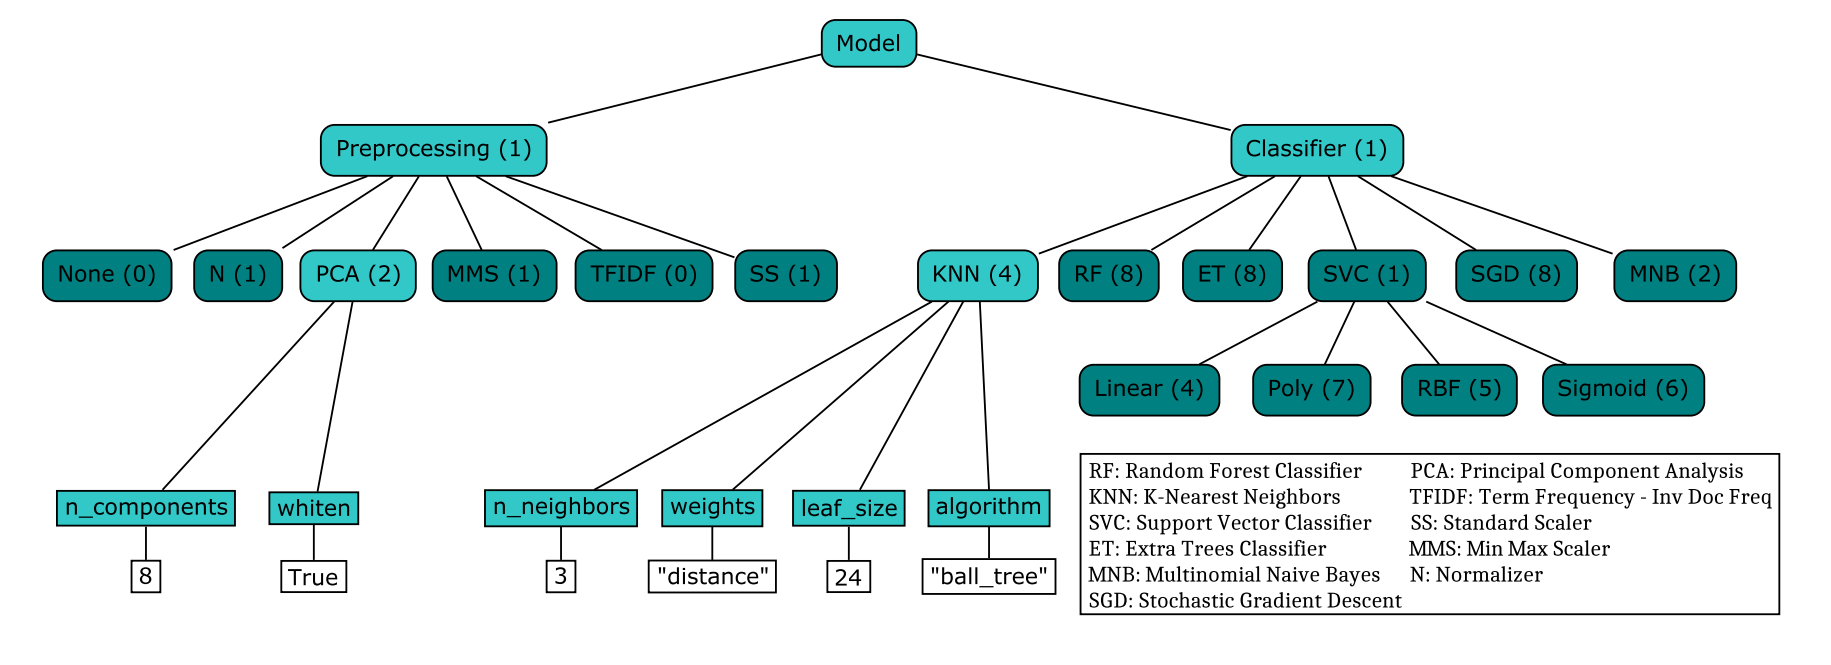
\includegraphics[width=1.0\textwidth]{images/cash}

\hfill Source: \lit{Komer et al. 2019}

\end{frame}
%----------------------------------------------------------------------
\section{Unbounded Configuration Spaces}
%----------------------------------------------------------------------
\begin{frame}[c]{Bounded Configuration Spaces}

So far, we assumed that each hyperparameter has a pre-defined domain.

\medskip
Problems:
\begin{itemize}
  \item for pipelines, we might don't know the size of the pipeline
	\begin{itemize}
		\item some components could be part of the pipeline multiple times
	\end{itemize}
  \pause
  \medskip
  \item sometimes we don't know a good range for a hyperparameter
  \begin{itemize}
     \item too large range $\leadsto$ very hard optimization problem
     \item too small range $\leadsto$ we might miss high-performance areas
  \end{itemize}

\end{itemize}

\pause
\bigskip

$\leadsto$ How can we design such configuration spaces?

\end{frame}
%----------------------------------------------------------------------
%----------------------------------------------------------------------
\begin{frame}[c, fragile]{Pipeline: Boolean Options}


\begin{verbatim}
  component_1 categorical {True, False}[True]
  component_2 categorical {True, False}[False]
  component_3 categorical {True, False}[False]
  ...
\end{verbatim}

\begin{itemize}
	\item Hard to optimize/not applicable if 
	\begin{itemize}
		\item we also have to find the ordering of the components
		\item if there is an upper bound on the number of components\\
		$\leadsto$ leads to many invalid configurations
		\item each component should be chosen more than once
	\end{itemize}
\end{itemize}

\end{frame}
%----------------------------------------------------------------------
%----------------------------------------------------------------------
\begin{frame}[c, fragile]{Pipeline: Fixed Pipelines Size}


\begin{verbatim}
step_1 categorical {comp1, comp2, comp3, ..., none}[comp1]
step_2 categorical {comp1, comp2, comp3, ..., none}[comp2]
step_3 categorical {comp1, comp2, comp3, ..., none}[none]
...
\end{verbatim}

\begin{itemize}
	\item encode each step of the pipeline with a choice between\\ all possible components
	\item Hard to optimize/not applicable if
	\begin{itemize}
		\item we don't know a good upper bound of the pipeline size
		\item there is an upper bound on how often a component can be chosen
	\end{itemize}
    \pause
    \bigskip
	\item If we don't need to specify the maximum length of the pipeline\\ this design is equivalent to search in a tree of possible pipelines
\end{itemize}

\end{frame}
%----------------------------------------------------------------------
%----------------------------------------------------------------------
\begin{frame}[c]{Pipeline: TPOT \litw{Olson et al. 2016}}

\centering
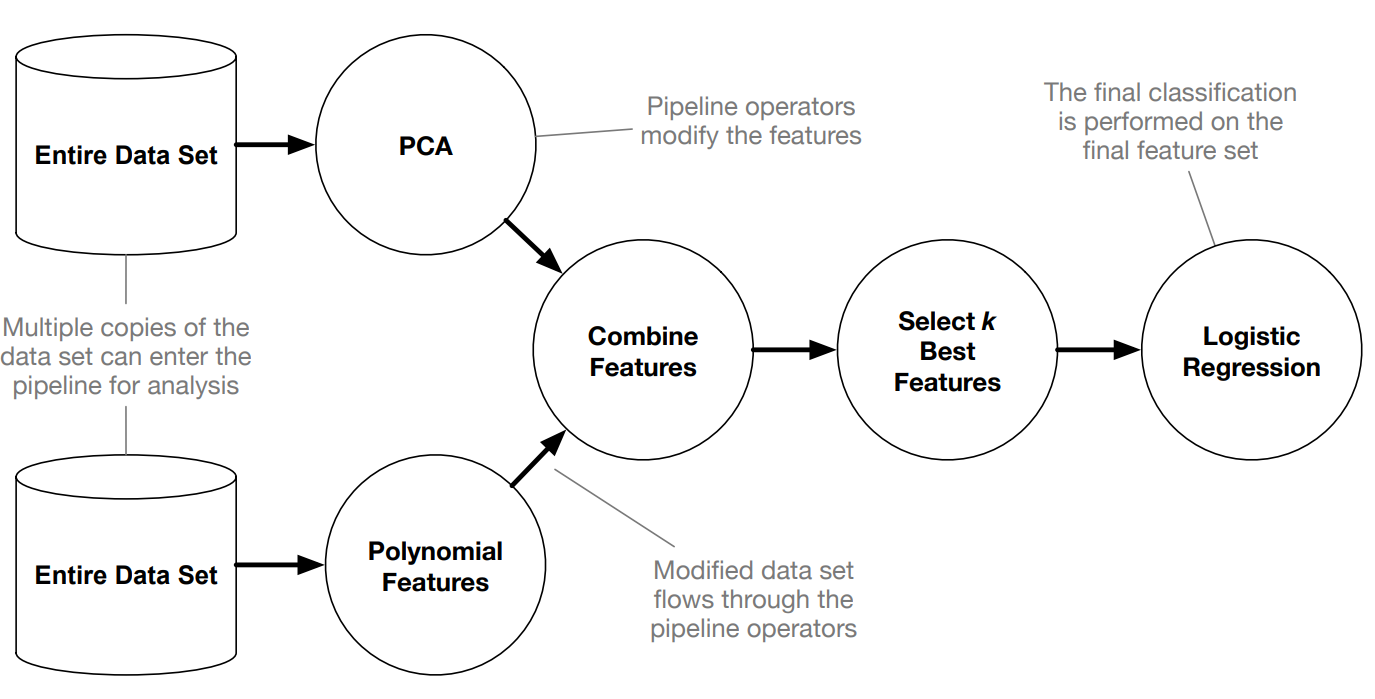
\includegraphics[width=0.8\textwidth]{images/tpot_tree}

\begin{itemize}
  \item TPOT searches in a space of tree-based pipelines
  \item Pipeline can potentially grow in size
  \item Challenge: avoid illegal pipelines
\end{itemize}

\end{frame}
%----------------------------------------------------------------------
%----------------------------------------------------------------------
\begin{frame}[c]{Bounds: Distributions instead of Bounds\\ (HyperOpt \litw{Bergstra et al. 2013})}

\begin{itemize}
  \item Instead of a range, HyperOpt also allows for user-defined distributions
  \begin{itemize}
    \item sampling of gamma (of SVM) could be done according to\\ log-normal distribution (with given statistics) 
  \end{itemize}
  \item Advantage:\\ allows for flexible definition of expert knowledge
  \item Disadvantage:\\ hard to find a good distribution if expert knowledge is limited
\end{itemize}

\end{frame}
%----------------------------------------------------------------------
%----------------------------------------------------------------------
\begin{frame}[c]{Bounds: Increasing Bounds \litw{Shahriari et al. 2015}}

\begin{enumerate}
  \item start with peaked distributions \\ s.t. it is very unlikely to sample outside of fairly narrow bounds
  \item increase width of distribution over time\\ to search in larger areas over time
\end{enumerate}

\bigskip
\pause

Remark:
\begin{itemize}
  \item similar ideas can be used for safe optimization
  \begin{itemize}
    \item quite important if a failed configuration incurs great (monetary) costs, \\
          e.g., a robot is destroyed because of its configuration \lit{Sui et al. 2015}
  \end{itemize}
\end{itemize}

\end{frame}
%----------------------------------------------------------------------
\section{Design Spaces for Neural Networks}
%----------------------------------------------------------------------
\begin{frame}[c]{Design of Neural Networks}

To train a deep neural network, we have many crucial design decisions \hands
\pause

\begin{itemize}
  \item number of layers
  \item number of neurons in each layer
  \item activation functions
  \item skip connections
  \item global architecture (MLP, ResNet, DenseNet, \ldots)
  \item regularization
  \begin{itemize}
    \item batch norm, weight decay, dropout, mixup, cut-out, \ldots 
  \end{itemize}
  \item optimizer hyperparameters
  \begin{itemize}
    \item type of optimizer (SGD, Adam, \ldots)
    \item learning rate
    \item momentum
    \item learning rate schedule
  \end{itemize}
  \item \ldots
\end{itemize}

$\leadsto$ joint global optimization of hyperparameters and architecture!

\end{frame}
%----------------------------------------------------------------------
%----------------------------------------------------------------------
\begin{frame}[c]{Neural Architecture Search (NAS)}

\begin{block}{Neural Architecture Search (NAS)}
Let
\begin{itemize}
  \item $\algo$ be a \alert{neural network}
  \item $\pcs$ be a design space\\ \alert{defining the architecture of a deep neural network}
  \item $D_{opt}$ be a training set which is split into $D_{train}$ and $D_{valid}$ 
  \item $\mathcal{L}(A_\conf, \dataset_{train}, \dataset_{valid})$ denote the loss of $A_\lambda$ trained on $D_{train}$ and evaluated on $D_{valid}$.
  
\end{itemize}
we want to find the architecture $\conf \in \pcs$ minimizing:
\begin{equation}
\conf^* \in \argmin_{\conf \in \pcs} \loss(\algo(\conf), \dataset_{train}, \dataset_{valid}) \nonumber
\end{equation}
\end{block}

\end{frame}
%----------------------------------------------------------------------
%----------------------------------------------------------------------
\begin{frame}[c]{Global NAS}

\centering
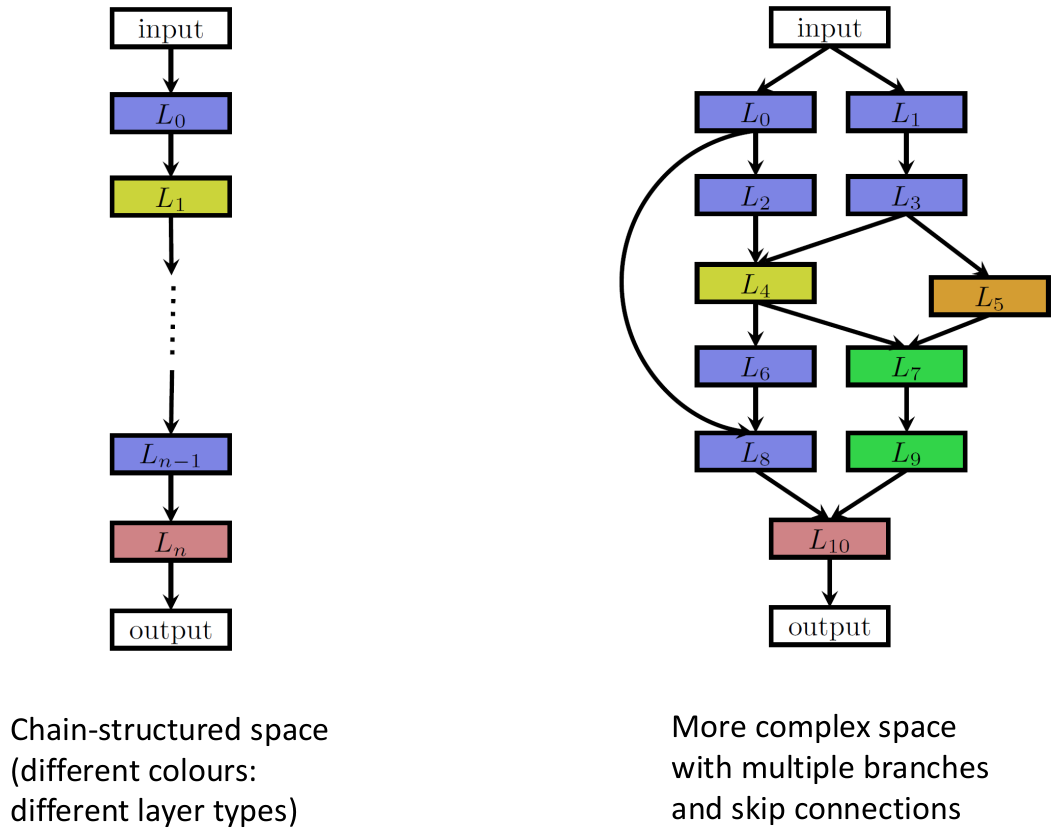
\includegraphics[width=0.7\textwidth]{images/nas_global.png}

\end{frame}
%----------------------------------------------------------------------
%----------------------------------------------------------------------
\begin{frame}[c]{Neural Architecture Search (NAS) -- Remarks}

\begin{itemize}
  \item yet another hyperparameter problem?
  \begin{itemize}
    \item[$\to$] we will see in later sessions how we exploit expert knowledge about neural networks to go beyond black-box HPO
  \end{itemize}
  \pause
  \bigskip
  \item Current practice: 
  \begin{itemize}
    \item hyperparameters (e.g., of the optimizer) are tuned manual or independently from the architecture
  \end{itemize}
  \pause
  \item Better practice:
  \begin{itemize}
    \item jointly optimize hyperparameters and architecture design\\ \lit{Zela et al. 2018}
  \end{itemize}
\end{itemize}

\end{frame}
%----------------------------------------------------------------------
%----------------------------------------------------------------------
\begin{frame}[c]{Shapes of Deep Neural Networks \litw{Kotila 2017}}

\begin{itemize}
  \item Many networks designed by humans follow a pattern
  \item Whether this is a good idea is not well studied
  \item Advantage: The number of hyperparameters is smaller
  \begin{itemize}
    \item E.g., instead of tuning the number of neurons in each layer\\ ($\leadsto$ one hyperparameter per layer),\\
          a few hyperparameters to define shape
  \end{itemize} 
\end{itemize}

\medskip
\centering
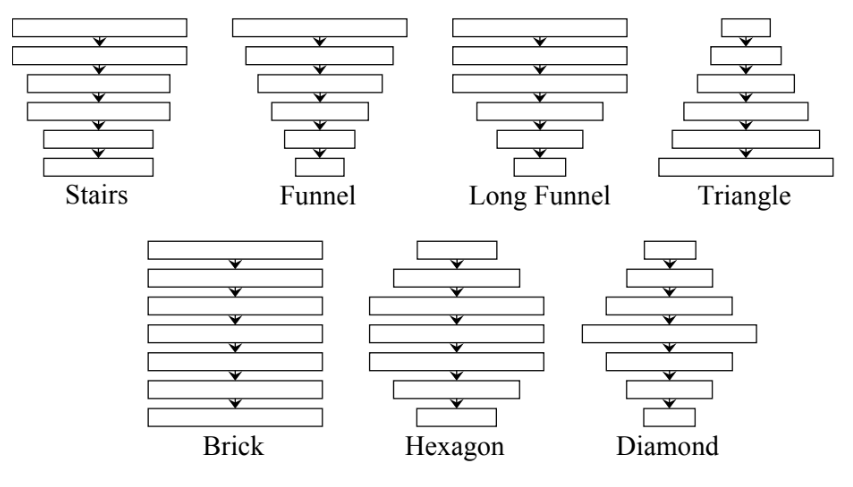
\includegraphics[width=.6\textwidth]{images/nas_shapes.png}

\end{frame}
%----------------------------------------------------------------------
%----------------------------------------------------------------------
\begin{frame}[c]{Cell NAS}

\centering
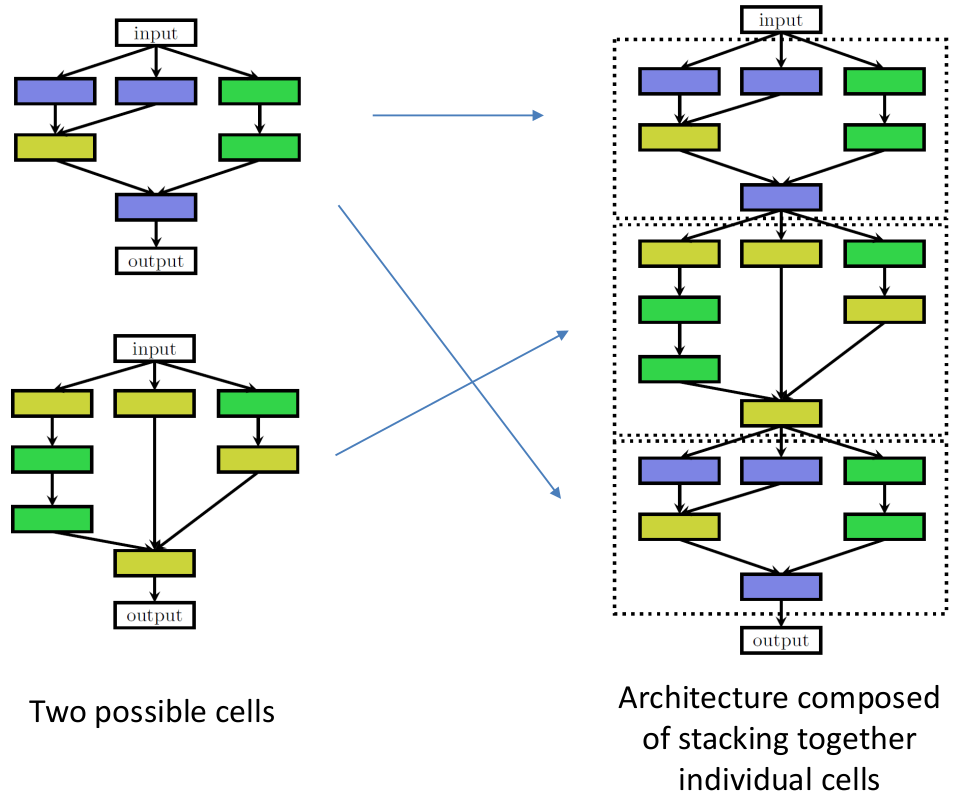
\includegraphics[width=0.7\textwidth]{images/nas_cellsearch.png}

$\leadsto$ Search for cells and repeat these in the final architecture $n$ times.

\end{frame}
%----------------------------------------------------------------------
%----------------------------------------------------------------------
\begin{frame}[c]{Flow of Tensors through Operators}


\begin{columns}
 \column{0.3\textwidth}

\centering
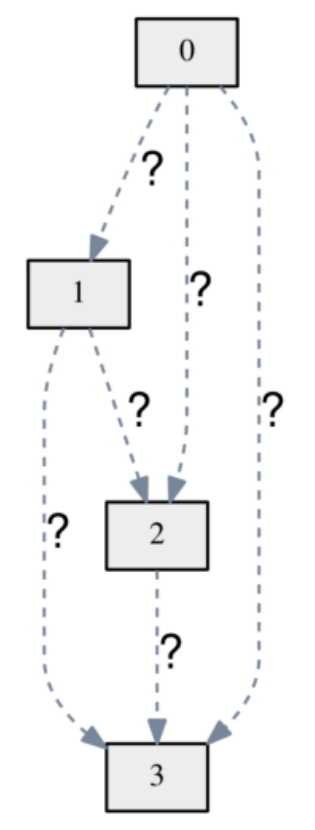
\includegraphics[width=0.6\textwidth]{images/nas_darts_space_idea.png}

 \column{0.7\textwidth}

\begin{itemize}
	\item each node is a tensor (i.e., a latent representation of the input data)
	\item between nodes operators change the data\\ (e.g., convolution or max pooling)
	\begin{itemize}  
		\item includes no-op operators to deactivate edges
	\end{itemize}
\end{itemize}


\begin{flushright}
	Source: \lit{Liu et al. 2019}
\end{flushright}

\end{columns}

\end{frame}
%----------------------------------------------------------------------
%----------------------------------------------------------------------
\begin{frame}[c]{Learning Goals}

Now, you should be able to \ldots

\begin{itemize}
  \item identify design decisions of machine learning algorithms
  \item explain different types of design decisions and there relations
  \item create design spaces
  \item discuss the pro and cons of different design space approaches
  \item explain design spaces for neural architecture search
\end{itemize}

\end{frame}
%----------------------------------------------------------------------
%----------------------------------------------------------------------
\begin{frame}[c]{Literature [These are links]}

\begin{itemize}
	\item \lit{\href{https://www.cs.ubc.ca/~hoos/Publ/Hoos10.pdf}{Programming by Optimization. Hoos 2012}}
	\item \lit{\href{https://ml.informatik.uni-freiburg.de/papers/13-KDD2013-AutoWEKA.pdf}{AutoWEKA and CASH. Thornton et al. 2013}}
	\item \lit{\href{https://www.automl.org/wp-content/uploads/2018/12/tpot.pdf}{TPOT. Olson and Moore. 2019}}
	\item \lit{\href{https://www.automl.org/wp-content/uploads/2018/12/hyperopt-sklearn-1.pdf}{Hyperopt-Sklearn. Komer et al. 2019}}
	\item \lit{\href{http://proceedings.mlr.press/v51/shahriari16.html}{Unbounded Bayesian Optimization via Regularization. Shahriari et al. 2016}}
	\item \lit{\href{https://arxiv.org/abs/1806.09055}{DARTS: Differentiable Architecture Search. Liu et al. 2019}}			
\end{itemize}

\end{frame}
%----------------------------------------------------------------------
